%  template.tex for Biometrics papers
%
%  This file provides a template for Biometrics authors.  Use this
%  template as the starting point for creating your manuscript document.
%  See the file biomsample.tex for an example of a full-blown manuscript.

%  ALWAYS USE THE referee OPTION WITH PAPERS SUBMITTED TO BIOMETRICS!!!
%  You can see what your paper would look like typeset by removing
%  the referee option.  Because the typeset version will be in two
%  columns, however, some of your equations may be too long. DO NOT
%  use the \longequation option discussed in the user guide!!!  This option
%  is reserved ONLY for equations that are impossible to split across 
%  multiple lines; e.g., a very wide matrix.  Instead, type your equations 
%  so that they stay in one column and are split across several lines, 
%  as are almost all equations in the journal.  Use a recent version of the
%  journal as a guide. 
%  
\documentclass[useAMS,usenatbib, referee]{biom}
%\documentclass[useAMS, usenatbib,usegraphicx]{biom}
%
%  If your system does not have the AMS fonts version 2.0 installed, then
%  remove the useAMS option.
%
%  useAMS allows you to obtain upright Greek characters.
%  e.g. \umu, \upi etc.  See the section on "Upright Greek characters" in
%  this guide for further information.
%
%  If you are using AMS 2.0 fonts, bold math letters/symbols are available
%  at a larger range of sizes for NFSS release 1 and 2 (using \boldmath or
%  preferably \bmath).
% 
%  Other options are described in the user guide. Here are a few:
% 
%  -  If you use Patrick Daly's natbib  to cross-reference your 
%     bibliography entries, use the usenatbib option
%
%  -  If you use \includegraphics (graphicx package) for importing graphics
%     into your figures, use the usegraphicx option
% 
%  If you wish to typeset the paper in Times font (if you do not have the
%  PostScript Type 1 Computer Modern fonts you will need to do this to get
%  smoother fonts in a PDF file) then uncomment the next line
%  \usepackage{Times}

%%%%% PLACE YOUR OWN MACROS HERE %%%%%

\def\bSig\mathbf{\Sigma}
\newcommand{\VS}{V\&S}
\newcommand{\tr}{\mbox{tr}}

%  The rotating package allows you to have tables displayed in landscape
%  mode.  The rotating package is NOT included in this distribution, but
%  can be obtained from the CTAN archive.  USE OF LANDSCAPE TABLES IS
%  STRONGLY DISCOURAGED -- create landscape tables only as a last resort if
%  you see no other way to display the information.  If you do do this,
%  then you need the following command.

%\usepackage[figuresright]{rotating}
\usepackage{amsmath}
\usepackage{graphicx}
% \usepackage{natbib}
% \usepackage{amsfonts}

%%%%%%%%%%%%%%%%%%%%%%%%%%%%%%%%%%%%%%%%%%%%%%%%%%%%%%%%%%%%%%%%%%%%%

%  Here, place your title and author information.  Note that in 
%  use of the \author command, you create your own footnotes.  Follow
%  the examples below in creating your author and affiliation information.
%  Also consult a recent issue of the journal for examples of formatting.

\title[]{Identifying Critical Shortcomings of Estimators of Discriminative Performance in Time-to-Event Analyses: A Comparison Study}

%  Here are examples of different configurations of author/affiliation
%  displays.  According to the Biometrics style, in some instances,
%  the convention is to have superscript *, **, etc footnotes to indicate 
%  which of multiple email addresses belong to which author.  In this case,
%  use the \email{ } command to produce the emails in the display.

%  In other cases, such as a single author or two authors from 
%  different institutions, there should be no footnoting.  Here, use
%  the \emailx{ } command instead. 

%  The examples below corrspond to almost every possible configuration
%  of authors and may be used as a guide.  For other configurations, consult
%  a recent issue of the the journal.

%  Single author -- USE \emailx{ } here so that no asterisk footnoting
%  for the email address will be produced.

%\author{John Author\emailx{email@address.edu} \\
%Department of Statistics, University of Warwick, Coventry CV4 7AL, U.K.}

%  Two authors from the same institution, with both emails -- use
%  \email{ } here to produce the asterisk footnoting for each email address

\author{Ying Jin$^{*}$\email{ying.jin@cuanschutz.edu} and
Andrew Leroux$^{**}$\email{andrew.leroux@cuanschutz.edu} \\
Department of Biostatistics and Informatics\\Colorado School of Public Health, 
University of Colorado-Denver Anschutz Medical Campus\\Aurora, CO, U.S.A.}

%  Exactly two authors from different institutions, with both emails  
%  USE \emailx{ } here so that no asterisk footnoting for the email address
%  is produced.

%  Three or more authors from same institution with all emails displayed
%  and footnoted using asterisks -- use \email{ } 

%\author{John Author$^*$\email{author@address.edu}, 
%Jane Author$^{**}$\email{jane@address.edu}, and 
%Dick Author$^{***}$\email{dick@address.edu} \\
%Department of Statistics, University of Warwick, Coventry CV4 7AL, U.K}

%  Three or more authors from same institution with one corresponding email
%  displayed

%\author{John Author$^*$\email{author@address.edu}, 
%Jane Author, and Dick Author \\
%Department of Statistics, University of Warwick, Coventry CV4 7AL, U.K}

%  Three or more authors, with at least two different institutions,
%  more than one email displayed 

%\author{John Author$^{1,*}$\email{author@address.edu}, 
%Kathy Author$^{2,**}$\email{anotherauthor@address.edu}, and 
%Wilma Flinstone$^{3,***}$\email{wilma@bedrock.edu} \\
%$^{1}$Department of Statistics, University of Warwick, Coventry CV4 7AL, U.K \\
%$^{2}$Department of Biostatistics, University of North Carolina at 
%Chapel Hill, Chapel Hill, North Carolina, U.S.A. \\
%$^{3}$Department of Geology, University of Bedrock, Bedrock, Kansas, U.S.A.}

%  Three or more authors with at least two different institutions and only
%  one email displayed

%\author{John Author$^{1,*}$\email{author@address.edu}, 
%Wilma Flinstone$^{2}$, and Barney Rubble$^{2}$ \\
%$^{1}$Department of Statistics, University of Warwick, Coventry CV4 7AL, U.K \\
%$^{2}$Department of Geology, University of Bedrock, Bedrock, Kansas, U.S.A.}


\begin{document}

%  This will produce the submission and review information that appears
%  right after the reference section.  Of course, it will be unknown when
%  you submit your paper, so you can either leave this out or put in 
%  sample dates (these will have no effect on the fate of your paper in the
%  review process!)

\date{{\it} . {\it } .  {\it
}.}

%  These options will count the number of pages and provide volume
%  and date information in the upper left hand corner of the top of the 
%  first page as in published papers.  The \pagerange command will only
%  work if you place the command \label{firstpage} near the beginning
%  of the document and \label{lastpage} at the end of the document, as we
%  have done in this template.

%  Again, putting a volume number and date is for your own amusement and
%  has no bearing on what actually happens to your paper!  

\pagerange{\pageref{firstpage}--\pageref{lastpage}} 
\volume{}
\pubyear{}
\artmonth{}

%  The \doi command is where the DOI for your paper would be placed should it
%  be published.  Again, if you make one up and stick it here, it means 
%  nothing!

\doi{}

%  This label and the label ``lastpage'' are used by the \pagerange
%  command above to give the page range for the article.  You may have 
%  to process the document twice to get this to match up with what you 
%  expect.  When using the referee option, this will not count the pages
%  with tables and figures.  

\label{firstpage}

%  put the summary for your paper here

\begin{abstract}
Predicting timing and occurrence of events of interest has been a major topic in biostatistical
research. While many estimators have been proposed to assess discriminative performance of time-to-event models, including time-dependent AUC and concordance, little work examined validity of these estimators, especially under the effect of data contamination or model overfit. In this paper, we aim to identify a previously unidentified feature of a class of popular estimators of discrimination in time-to-event models that can result in vastly over-optimistic out-of-sample discrimination. As a result, we find this class of estimators inappropriate for use in model assessment and selection based on out-of-sample evaluation criteria (e.g. cross-validated discrimination). Another class of non-parametric estimators of discrimination does not suffer from this problem, but are highly variable. We propose alternative estimators which smooth non-parametric estimators using penalized regression splines, reducing variability of non-parametric time-varying estimates of discrimination while retaining proper out-of-sample behavior. We illustrate the behavior of both existing estimators and our proposed estimators in a simulation study and a real-world data application. 
\end{abstract}

%  Please place your key words in alphabetical order, separated
%  by semicolons, with the first letter of the first word capitalized,
%  and a period at the end of the list.
%

\begin{keywords}
Concordance; C-index; Proportional hazard model; Model selection; Survival prediction; Time-dependent AUC
\end{keywords}

%  As usual, the \maketitle command creates the title and author/affiliations
%  display 

\maketitle

%  If you are using the referee option, a new page, numbered page 1, will
%  start after the summary and keywords.  The page numbers thus count the
%  number of pages of your manuscript in the preferred submission style.
%  Remember, ``Normally, regular papers exceeding 25 pages and Reader Reaction 
%  papers exceeding 12 pages in (the preferred style) will be returned to 
%  the authors without review. The page limit includes acknowledgements, 
%  references, and appendices, but not tables and figures. The page count does 
%  not include the title page and abstract. A maximum of six (6) tables or 
%  figures combined is often required.''

%  You may now place the substance of your manuscript here.  Please use
%  the \section, \subsection, etc commands as described in the user guide.
%  Please use \label and \ref commands to cross-reference sections, equations,
%  tables, figures, etc.
%
%  Please DO NOT attempt to reformat the style of equation numbering!
%  For that matter, please do not attempt to redefine anything!

\section{Introduction}
\label{s:intro}


Modelling time to event outcomes, often referred to as survival analysis, is a major area of methodologic development in biostatistical research. Broadly, model performance is evaluated using discrimination or calibration criteria, with the former criteria being similar to area under the receiver operating characteristic curve (AUC) for binary outcomes. While several estimators have been proposed to assess discriminative performance of time-to-event models, including time-dependent AUC and concordance, there exists a previously unidentified feature of a class of these estimators which renders them inappropriate for use in many contexts. Specifically, semi-parametric estimators have a previously unidentified potential to substantially overestimate out-of-sample discriminative performance even when the model is correctly specified. In this paper, we identify the source of this phenomena and illustrate the poor behavior of this class of semi-parametric estimators in the context of a simulation study and data application. Additionally, we propose alternative non-parametric estimators to be used in practice that do not overestimate out-of-sample discriminative performance.

% Evaluators of dicrimination

Accuracy of discrimination of risk in time-to-event models can be assessed locally (i.e. for a fixed time point) or globally (summarized over a set of time points). Local discrimination involves defining a set of ``cases" and ``controls" based on the event of interest, and then calculating the corresponding receiver operating characteristic (ROC) curve that is specific to the time point. The local area-under-the-ROC-curve (AUC) are broadly referred to as time-varying AUC, with two popular estimands being Incident/Dynamic AUC and Cumulative/Dynamic AUC \citep{hz2005}. The former compares discrimination of risk for incident events and the latter focuses on historical events. Global summaries of discrimination are generally referred to as measures of Concordance \citep{Harrell1996}. Both local and global measures assess how well estimated risk compares to observed event times, accounting for censoring. In this paper we restrict our focus to estimators of Incident/Dynamic AUC and Concordance of time-to-event outcomes with independent right censoring conditional on covariates.

% flaws of existing estimator
It has been previously noted that semi-parametric estimators of discrimination designed for data generated according to a Cox proportional hazards model are inaccurate and potentially over-optimistic when the proportional hazards assumption is violated \citep{Schmid2013}. Here, we identify different and potentially more worrisome behavior of the same semi-parametric estimators that can occur even under a correctly specified proportional hazards model. The poor behavior of semi-parametric estimators is most easily seen in the context of: 1) model overfit, and 2) contaminated data. Both are common issues when developing models based on existing real-world data. Overfit can happen when the model is too complicated with too many free parameters or noise signals, for which out-of-sample evaluation is often used to evaluate model generalizability. However, as shown in following sections, semi-parametric estimators also overestimate out-of-sample discriminative performance, even more severely than in-sample. Data contamination, on the other hand, happens when the dataset is collected with outlying or noisy obervations. In both cases, the semi-parametric estimators show over-optimistic discriminative performance when the underlying model in fact fits poorly. 

% some reason behind 
Measures of discrimination have been, and continue to be, used frequently for assessment of model performance, both for binary and time-to-event outcomes, despite the fact that these measures may be strongly disconnected from accuracy of predictions \citep{lobo2008}. That is, discrimination is only supposed to tell us whether our model {\it ranks} subjects' risks correctly, but says nothing about the {\it accuracy} of risk estimation or prediction (e.g. probability of an event). Indeed, compelling arguments have been made that discrimination is an inappropriate criteria for model selection in the context of time-to-event models \citep{blanche2018}. Nevertheless, measures of discrimination provide one piece of useful information about the predictions made by a particular model and, due to their utilization by practitioners, understanding the properties of various estimators is critical. Thus, we add to the literature by identifying both the phenomena of inflated out-of-sample estimation of discriminative performance and the mechanism by which it occurs in semi-parametric estimators. In addition, we provide recommendations for alternative non-parametric estimators for performance assesment and model selection.

% following content
To address our key goals, we designed and implemented a simulation study comparing multiple semi-parametric and non-parametric estimators of both Incident/Dynamic AUC and Concordance under a Cox regression framework. Specifically, we simulate data using a Cox proportional hazards model with three true predictors and a Weibull baseline hazard for 500 individuals, later splited into a training and a testing set. To investigate the effect of model overfit, we then fit three separate models on the training set: a correctly specified model and two models with either twenty or one hundred random noise signals, introducing various degrees of model overfit. As for the effect of data contamination, we introduce outliers to test samples whose covariates follow different distribution from the original samples. The comparison between in-sample and out-of-sample estimates shows that semi-parametric estimators vastly overestimate the discriminative performance in both situations. However, non-parametric estimators, despite achieving the desired behavior of correctly reflecting the out-of-sample discriminative performance, are highly unstable. Thus, we propose to smooth the estimators using additive regression models. 

The difference between estimators are also illustrated using an application to the 2011-2014 National Health and Nutrition Examination Survey (NHANES) data, where we fit an additive Cox model with covariates modelled using 200 basis functions, and a simple linear cox model. The result is a clearly overfit model where out-of-sample discrimination is estimated to be implausibly high using semi-parametric estimators, while non-parametric estimators assess model discrimination to be appropriately low. 


\section{Method}
\label{s:method}


Let $i = 1,\ldots, N$ denote individual, and $T_i^*$ denote a non-negative random variable (e.g. time-to-event) subject to right censoring. For each individual $i$ we observe $[T_i, \delta_i, \bmath{X}_i^t]$ where $T_i = min(T_i^*, C_i)$ is the observed time (minimum of censoring time $C_i$ and true event time $T_i^*$). $\delta_i = 1(T_i^* \leq C_i)$ is the event indicator, and  $\bmath{X}_i \in R^p$ is a vector of time-fixed covariates. We assume $C_i$ is independent of event time $T_i^*$ conditional on $\bmath{X}_i$. Additionally, the data is assumed to be generated by the proportional hazards model \citep{cox1972}, where the log hazard of the event time process takes on the additive form
\[
\log \lambda(t|\bmath{X}_i) = \log \lambda_0(t) + \bmath{X}_i^t \bmath{\beta}\
= \log\lambda_0(t) + \eta_i; \hspace{0.5cm} t > 0 \;.
\]

In the proportional hazards model, $\log \lambda(t|\bmath{X}_i)$ is the conditional log-hazard for subject $i$ given their covariate vector $\bmath{X}_i$, and $\log \lambda_0(t)$ is the log baseline hazard which is constant across subjects. $\bmath{\beta}$ is a vector of unknown parameters, corresponding to the linear contribution of each element of $\bmath{X}_i$ to the log hazard, and $\eta_i$ is the overall contribution of covariates to log hazard, indicating the subject-specific deviation of log hazard from the population average ($\log \lambda_0(t)$). Hereafter we refer to $\eta_i$ as a risk score for subject $i$. 


\subsection{Measures of Discrimination for Time-to-event Models}
\label{subsec:methods_estimands}

As discussed in Section \ref{s:intro}, there are a number of measures developed for assessing the discriminative ability of time-to-event models. This work focuses on two estimands, one of which measures local (i.e. time-specific) discrimination, and the other is a corresponding global (i.e. averaged across time points) measure of discrimination. Specifically, we consider the local measure Incident/Dynamic area-under-the-curve ($AUC^{I/D}(t)$) and the global measure Concordance \citep{Harrell1996} ($C$), a weighted average of $AUC^{I/D}(t)$ over time. In this section we define the two estimands, then in Section \ref{subsec:methods_estimators} we introduce various estimators of $AUC^{I/D}(t)$ and $C$.

\subsubsection{Incident/Dynamic AUC}
\label{par:define_auc}

Incident/Dynamic AUC, or $AUC^{I/D}(t)$ \citep{hz2005}, generalizes the notion of area under the ROC curve for binary data, allowing for time-dependent discrimination in time-to-event models. This is achieved by defining sets of cases (incident events at $T_i^* = t$) and controls (individuals with $T_i^* > t$) specific to time t, calculating the corresponding incident sensitivity and dynamic specificity at a series of unique thresholds for risk score ($\eta_i$), deriving a time-specific ROC curve and estimating the area under it. As with AUC for binary data, $AUC^{I/D}(t) \in [0,1]$, with values closer to $1$ indicating better discrimination and values near $0.5$ indicating the risk score $\eta_i$ is no better at discriminating events at time $t$ than a flip of a coin. We describe these estimands in more detail below. 

Incident sensitivity and dynamic specificity are defined as
\[
    sensitivity^{I}(c,t) = {TP}_t^{I}(c) = Pr(\eta_i > c|T_i^* = t)
\]
\[
    specificity^{D}(c,t) = 1-FP_t^{D}(c) = Pr(\eta_i \leq c|T_i^* > t) 
\]

where $TP^I$ and $FP^D$ are abbreviations for time-specific incident true-positive and dynamic false-positive rate respectively, and $c$ is a threshold of risk score $\eta_i$. Using the above definitions for incident sensitivity and dynamic specificity, we can then define the Incident/Dynamic ROC curve. Let p denote a dynamic value of $FP_t^{D}(c)$, then 
\[
ROC_t^{I/D}(p) = TP_t^{I}\{[FP_t^{D}]^{-1}(p)\}
\]

From which it follows that $AUC^{I/D}(t)$: 
\[
   AUC^{I/D}(t) = \int_0^1 ROC_t^{I/D}(p)dp
\]

In practice $AUC_t^{I/D}(t)$ is generally approximated by numeric integration, evaluating \\$[TP_t^{I}(c), FP_t^{D}(c)]$ for $c \in \{\eta_i: 1 \leq i \leq N\} \cup -\infty$. 

\subsubsection{Concordance}
\label{par:define_c}

Concordance, defined as $C = Pr(\eta_i < \eta_j| T_i^* > T_j^*)$, represents the overall agreement between observed event times and risk scores. As with $AUC^{I/D}(t)$, $C \in [0,1]$, with values closer to $1$ denoting better global discrimination of the risk score. In practice, $T_i^*$ may have support beyond the duration of a study, resulting in a need to administratively censor participants at some follow-up time $\tau$ (e.g. the end of the study). In the context of administrative censoring, the estimand becomes $C^\tau = Pr(\eta_i < \eta_j| T_i^* > T_j^*, T_j^* < \tau)$. It has been shown that this truncated concordance is a weighted-average of Incident/Dynamic AUC \citep{hz2005}:
\[
C^\tau = \int_0^{\tau} 
AUC^{I/D}(t)w^{\tau}(t)dt;
\hspace{0.5cm}
w^{\tau}(t) = \frac{2f(t)S(t)}{1-S^2(\tau)}
\]
where $S(t)$ is the marginal survival function of event times (not conditional on covariates) and $f(t)$ is the marginal probability density function of time to event. 

\subsection{Estimators of Discrimination for Time-to-event Models}
\label{subsec:methods_estimators}

In this section we discuss methods of estimating $AUC^{I/D}(t)$ and $C^\tau$ as defined in Section~\ref{subsec:methods_estimands} above. We distinguish between semi- and non-parametric estimators as the different classes of estimators with regard to both their formulation and out-of-sample behavior.

\subsubsection{Incident/Dynamic AUC} 
\label{par:est_auc}

As mentioned in Section~\ref{subsec:methods_estimands}, estimation of  $AUC^{I/D}(t)$ can be achieved by numeric approximation of the integral of the Incident/Dynamic ROC curve at time $t$. Procedurally, this is done by obtaining estimates of incident sensitivity and dynamic specificity at all thresholds $c \in \{\eta_i: T_i \geq t\} \cup -\infty $, which is the set of unique values of individual risk score of subjects at risk at time $t$. Evaluating at $c = -\infty$ ensures the estimated $ROC_t^{I/D}$ passes through the point $(1,1)$. Thus, different estimators of $AUC^{I/D}(t)$ arise from the use of different estimators for dynamic specificity and/or incident sensitivity. Here, all estimators considered use the same non-parametric estimator of dynamic specificity, but differ in their approach to estimate incident sensitivity. 

Specifically, suppose we have obtained estimated coefficient $\hat{\bmath{\beta}}$ and used it to estimate individual risk scores $\hat{\eta}_i = \bmath{X}_i^t\hat{\bmath{\beta}}$.  Dynamic specificity then can be estimated 
 as follows: 
\begin{equation}
1-\widehat{specificity}^{D}(c,t)= \hat{FP}_t(c) = 
\frac{\sum_{k}I(\hat{\eta}_k>c)I(T_k>t)}{\sum_{j}I(T_j>t)}
\label{eq:spec_np} 
\end{equation}

This estimator of dynamic false-positive rate is built based on the plug-in principal, counting up the proportion of individuals who have an estimated risk greater than a particular threshold among those individuals who have not experienced the event by time $t$.

Moving on to estimators of incident sensitivity, first consider a non-parametric estimator based similarly on the plug-in principal:

\begin{equation}
\widehat{sensitivity}^{I}(c,t)=
\hat{TP_t}^{NP}(c)=  \frac{\sum_{k}I(\hat{\eta}_k>c)I(T_k=t)I(\delta_k=1)}{\sum_{j}I(T_j=t)I(\delta_j=1)}    
\label{eq:sens_np} 
\end{equation}

This non-parametric estimator is not continuous over time because it needs to be evaluated at time points with more than one event ($\{t: \sum_{j}I(T_j=t)I(\delta_j=1) > 0\}$), and the resulting $ROC_t^{I/D}(p)$ is a step function. This estimator is inherently more variable than the non-parametric estimator of dynamic specificity in Equation (\ref{eq:spec_np}). To see this, note that Equation (\ref{eq:sens_np}) is based on counting the proportion of individuals who have a risk score above a particular threshold $c$ among those with an observed event at $t$. In practice there is often only one event at a single time point, and the estimated value of sensitivity would fluctuate between 0 and 1. 

Then consider the semi-parametric estimator of $AUC^{I/D}(t)$ proposed by \citet{hz2005}. It uses the same non-parametric estimator of $\hat{FP}_t(c)$ in Equation (\ref{eq:spec_np}), but differs in their estimator of incident sensitivity:

\begin{equation}
\hat{TP_t}^{SP}(c)=\frac{\sum_{k}I(\hat{\eta}_k>c)I(T_k\geq t)exp(\hat{\eta}_k)}{\sum_{j}I(T_j\geq t)exp(\hat{\eta}_j)}
\label{eq:sens_sp}
\end{equation}

Instead of counting the proportion of true-positive subjects, this estimator conditions on all subjects at risk at time $t$ and weigh the subjects by their exponential estimates of risk score. The subject-specific weight $\frac{exp(\hat{\eta}_k)}{\sum_{j}I(T_j\geq t)exp(\hat{\eta}_j)} $ depends on coefficient estimates $\hat{\bmath{\beta}}$, thus "parametric" in nature. In addition, we note the lack of dependence on actual observed events at $t$ (i.e. $\delta_i$ appears nowhere in this formula). The above two points are the key marks to distinguish the formulation between non- and semi-parametric estimators. They are also the reasons that semi-estimators, though consistent under our proposed framework \citep{10.2307/2680613} and relatively smooth in practice, suffer from over-optimistic inflation. 

\subsubsection{Concordance}
\label{par:est_c}

Truncated concordance, $C^{\tau}$, may be estimated using the result linking $C^{\tau}$ to $AUC^{I/D}(t)$ (weighted average) or using other semi- and non-parametric estimators. First consider estimating $C^{\tau}$ as the weighted integral of $AUC^{I/D}(t)$. This can be done using either non- or semi-parametric estimates of $AUC^{I/D}(t)$, with weights derived from estimated marginal survival function: $\hat{w^{\tau}}(t) = \frac{2\hat{f}(t)\hat{S}(t)}{1-\hat{S}^2(\tau)}$. However, as was mentioned previously, the non-parametric estimator of $AUC^{I/D}(t)$ derived from Equations (\ref{eq:spec_np}) and (\ref{eq:sens_np}) is highly variable, which presents a challenge for numeric integration. We therefore propose to smooth the non-parametric $\hat{AUC}^{I/D}(t)$ using penalized regression splines via the \textit{mgcv} package \citep{wood2003, wood2011, wood2017} in \textit{R} \citep{Rsoftware}.
\[
    \hat{AUC}^{I/D}(t) = 
    \tilde{AUC}^{I/D}(t) + \epsilon(t) =
    \sum_{k=1}^K \xi_k B_k(t) + \epsilon(t)
\]

Here $\tilde{AUC}^{I/D}(t)$ is the smoothed Incident/Dynamic AUC estimates, modelled as the linear combination of a set of cubic spline basis functions $B_1(t)...B_K(t)$ subject to penalty on second derivative. $\epsilon(t)$ denotes a random noise that follows a zero-mean Gaussian process across time. Other options, such as kernel smoothing \citep{VANGELOVEN2021107095} are possible. 

Please note that the weight estimator $\hat{w^{\tau}}(t)$ requires estimating both marginal survival function $\hat{S}(t)$ and density of survival time $\hat{f}(t)$. While Kaplan-Meier curve is commonly used to estimated $S(t)$, it is unrealistic to estimate $f(t)$ by taking the derivative of $\hat{S}(t)$, since $\hat{S}(t)$ would be a step function. Therefore, it has also been proposed to use a smoothed version of Kaplan-Meier curve. In this paper, we use a Constrained Additive Model \citep{pya2021}: 

\[
\hat{S}(t) = \tilde{S}(t) + \epsilon(t)
    = \sum_{k=1}^K \zeta_k M_k(t) + \epsilon(t)
\]

where $\hat{S}(t)$ is the Kaplan-Meier estimators of marginal survival function, and smoothed survival function $\tilde{S}(t)$ is modelled as a linear combination of P-spline basis functions $M_1(t)...\\M_K(t)$ that are subject to the following constrains:
\begin{enumerate}
    \setlength\itemsep{0em}
    \item Monotonicity: $\tilde{S}(t_1) > \tilde{S}(t_2)$ for $t_1 < t_2$
    \item $\tilde{S}(0) = 1$
    \item Positivity: $\tilde{S}(t) > 0$
\end{enumerate}

and $\epsilon(t)$ is a random noise that follows a zero-mean Gaussian process across time, similar to the smoothing of non-parametric $\hat{AUC}^{I/D}(t)$. 

We hereafter refer to the estimator of concordance derived from non-parametric $\hat{AUC}^{I/D}(t)$ as non-parametric concordance $\hat{C}_{NP}$, likewise estimator from the $\hat{AUC}^{I/D}(t)$ by  Heagerty \& Zheng as the semi-parametric concordance $\hat{C}_{SP}$. 
The estimator by integrating $\tilde{AUC}^{I/D}(t)$, the smoothed non-parametric estimator of Incident/Dynamic AUC, will be referred to as smoothed non-parametric concordance $\hat{C}_{SNP}$. 
In addition to estimators of Concordance based on integrating estimates of $AUC^{I/D}(t)$, we consider one additional semi-parametric estimator proposed by \citet{gh2005}
\[
\hat{C}_{GH} = \frac{2}{n(n-1)}\sum_{i<j}{\frac{I(\hat{\eta}_j-\hat{\eta}_i<0)}{1+exp(\hat{\eta}_j-\hat{\eta}_i)}+\frac{I(\hat{\eta}_i-\hat{\eta}_j<0)}{1+exp(\hat{\eta}_i-\hat{\eta}_j)}}
\]

and one additional non-parametric estimator of \citet{Harrell1996}
\[
\hat{C}_{Harrell} = 
\frac{\sum_{i<j}I(T_i<T_j)I(\hat{\eta}_i>\hat{\eta}_j)I(\delta_i=1)+I(T_i>T_j)I(\hat{\eta}_i<\hat{\eta}_j)I(\delta_j=1)}{\sum_{i<j}I(T_i<T_j)I(\delta_i=1)+I(T_i>T_j)I(\delta_j=1)} 
\]


Similar to the semi-parametric estimator of dynamic sensitivity, the semi-parametric estimator of Concordance proposed by \citet{gh2005} includes terms of the form $e^{\eta}$ and excludes event status $\delta$, while Harrell's C only compares relative ranking of risk estimation. In addition, we note that it is known that Harrell's C is biased for the estimand of interest in the presence of censoring. Alternative unbiased estimators have been proposed by \citet{Uno2011}, but we use Harrell's C here for simplicity of presentation. 

\subsection{Mechanism for Inflated Estimation of Out-of-Sample Discrimination}
\label{subsec:methods_mechanism}

As mentioned in the introduction, semi-parametric estimators are prone to overestimate true model performance on new samples, even when the model is correctly specified. To understand the mechanism behind this critical flaw, we need to revisit the formula of semi-parametric estimator of true positive rate:

\begin{equation}
\hat{TP}_t^{SP}(c) 
=\frac{\sum_{k}I(\hat{\eta}_k>c)I(T_k\geq t)exp(\hat{\eta}_k)}{\sum_{j}I(T_j\geq t)exp(\hat{\eta}_j)} =\sum_{k}I(\hat{\eta}_k>c)I(T_k\geq t)\frac{exp(\hat{\eta}_k)}{\sum_{j}I(T_j\geq t)exp(\hat{\eta}_j)} 
\label{eq-weight}
\end{equation}


While counting the number of observations at risk at time t with risk score over a threshold c, this estimator also weighs observations by the exponential of their estimated risk scores, $\frac{exp(\hat{\eta}_k)}{\sum_{j}I(T_j\geq t)exp(\hat{\eta}_j)}$. Therefore, the true positive rate estimates depend heavily on the value of $\hat{\eta}$ of subjects at risk, regardless of whether the risk is correctly estimated or whether an event actually happened to the subjects at the specific time point. This lack of dependence on actual observation is illustrated in Figure~\ref{fig-outlier}. In this example, we present two ROC curves from the same model on two datasets derived from the semi-parametric estimator of sensitivity at a specific time point. The two datasets are identical except for one subject: The dataset represented by the yellow line introduced one outlier with a large risk score $\hat{\eta}$. As is revealed, this one observation has driven out-of-sample AUC to 99.8\% through the weight term at a single time point, while it in fact had no contribution to the discriminative ability of the underlying model. 

% outlier
\begin{figure}
\centerline{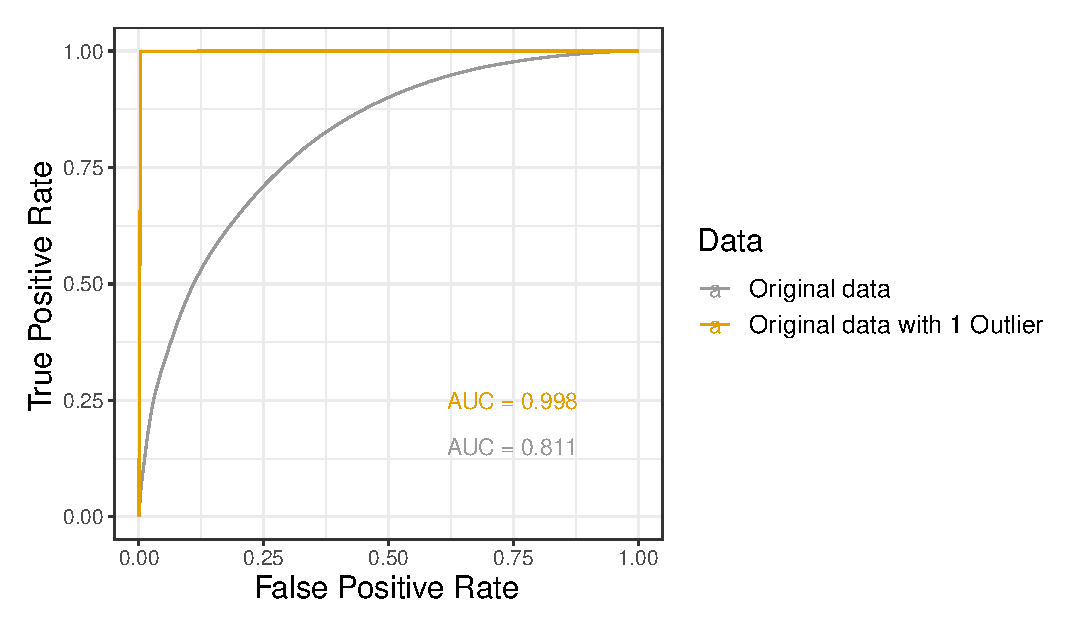
\includegraphics[width=0.8\textwidth]{outlier_exp.eps}}
% 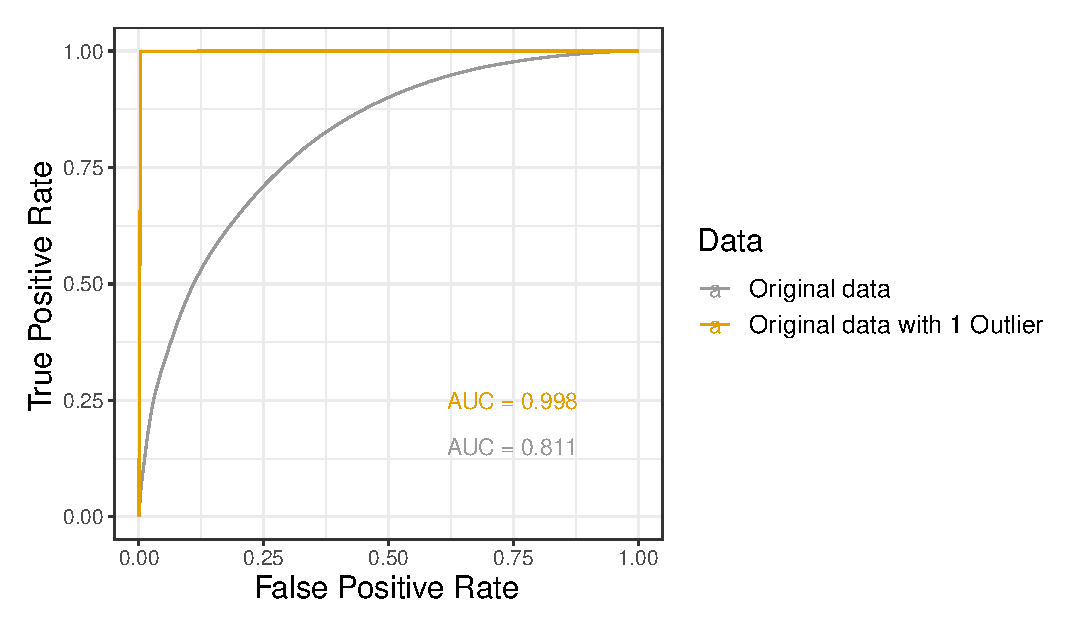
\includegraphics[width=0.7\textwidth]{outlier_exp.eps}
\caption{Change of out-of-sample semi-parametric estimation of discriminative performance after introducing one outlier. The dataset represented by the yellow line has the same observations with the grey line, except for one outlier with a large risk score.}
\label{fig-outlier}
\end{figure}


In practice, we can expect this phenomena to occur in at least two situations: 1) the model ovefits to the collected sample; or 2) the sample is contaminated with outlying observations. In both cases, the estimated risk score $\hat{\eta}$ can be highly variable, imposing too much importance on some observations and neglecting the others through the weight term in Equation (\ref{eq-weight}). 

\section{Simulation Study}
\label{sec:simulation}

We performed a simulation study to illustrate the behavior of the various estimators of discrimination presented in Section~\ref{subsec:methods_estimators}, aimed to provide a comparison of in- versus out-of-sample behavior in finite samples. As such, we generate data under a single data generating mechanism according to a Cox proportional hazards model with independent censoring, a framework under which each semi- and non-parametric estimator of $AUC^{I/D}(t)$ considered here are unbiased and consistent. 

The specific scenario we consider uses a true data generating mechanism of the Proportional Hazards model with three covariates $\bmath{X} = (X_1, X_2, X_3)$ simulated as independent $N(0,1)$ random variables. Each individual's risk is then 
\begin{equation}
    \log \lambda(t|\bmath{X}) 
    = \log \lambda_0(t) + \bmath{X}^t\bmath{\beta} 
    = \log(p\theta t^{p-1})+\eta, \hspace{0.3cm} t>0 
\label{eq:sim_model}
\end{equation}

with $\bmath{\beta} = (1, -1, 0.25)$ and Weibull baseline hazard $\lambda_0(t) = p\theta t^{p-1}$, $[\theta, p]^t = [2, 2]^t$. Censoring times are simulated uniformly from two discrete values $(0.5,1)$ independently of event times, with administrative censoring for all individuals at $\tau=1$.

We simulate $1000$ datasets containing $N=250$ individuals used for model fitting and evaluation of estimated in-sample discrimination (the training set). An additional $250$ individuals are simulated for each dataset under the same data generating mechanism in Equation ~(\ref{eq:sim_model}) to evaluate estimated out-of-sample discrimination (the testing set). The behavior of semi- and non-parametric estimators is compared under the two scenarios mentioned in Section~\ref{subsec:methods_mechanism}: model overfit and data contamination. 

Model overfit is introduced by adding noise signals when fitting models on the training set. These noise signals are generated independently from both covariates and the time-to-event outcomes, thus should not improve the discriminative ability of fitted models. To introduce different severity of overfit, we construct three different models: 1) a correctly specified model with no noise signals; 2) a moderately overfitted model with $20$ noise signals; and 3) a much overfitted model with $100$ noise signals. In some rare cases, number of covariates included in the model exceeded the number of total events, causing non-convergence issues during model fitting. To address this issue, we incorporated a convergence check that excludes such datasets from the simulation process. 

In the second scenario, the training datasets are also generated from Equation ~(\ref{eq:sim_model}). However in the testing set, we introduce 10\% of contaminated observations whose covariates are generated from a different distribution. Specifically, we study the effect on out-of-sample behaviour of two different types of data contamination: 1) a mean shift, where the covariates are generated from $N(5, 1)$; and 2) a spread change, where covariates are generated from $N(0, 5)$. Since these contaminated observations are not used for model fitting, they should not contributed to the discrimitive ability of models fitted on the training sets. We would expect the models to predict these observations poorly, causing low out-of-sample estimates of Incident/Dynamic AUC and concordance.


\subsection{Model overfit}
\label{sec:sim_overfit}

Figure \ref{fig:overfit} presents the in-sample and out-of-sample estimates of model discrimination ability across simulated datasets under different degrees of model overfit. Estimated $AUC^{I/D}(t)$ is visualized in (a), smoothed across all simulations for better visual presentation, since these estimated values tend to be highly variable especially for the non-parametric and smoothed non-parametric estimators. The color of curves indicates different models, including the correctly specified model (grey), a moderately overfit model (yellow), and a highly overfit model (blue).
Solid lines represent in-sample estimates and dashed lines out-of-sample estimates. The black solid lines is the true values of $AUC^{I/D}$ derived from the data generating scheme. Estimated concordance is presented in (b), with grey boxes for in-sample and yellow out-of-sample estimates. The black, horizontal solid line is the true value of concordance. 

\begin{figure}
\centering
\includegraphics[width=\textwidth]{fit_overfit.eps}
\caption{Behavior of estimators of model discrimination under the effect of model overfit.  Estimates of Incident/Dynamic AUC are presented in (a), where solid lines represent in-sample estimates and dashed lines represent out-of-sample estimates. Color of lines indicates the underlying model, where grey corresponds to the correctly specified model, yellow a moderately overfit model with 20 noise signals, blue a highly overfit model with 100 noise signals. The solid black line represents true value of AUC. Estimates of concordance are presented in (b) with grey indicating in-sample and yellow out-of-sample estimates. The black horizontal line is the true value of concordance.}
\label{fig:overfit}
\end{figure}

In the scenario where a model is overfit to the data, we would expect the in-sample estimators to overestimate while the out-of-sample estimators to underestimate the discriminative performance due to poor generalization for both local and global evaluation metrics. In addition, we would expect the severity of in-sample overestimation/out-of-sample underestimation to increase with increasing model overfit. Visually, in Figure \ref{fig:overfit} this would correspond to solid lines being higher and dashed lines being lower than the black line in (a), and grey boxes being higher and yellow boxes being lower than the black line in (b). This is clearly the case for non-parametric and smoothed non-parametric estimators, but flipped for the semi-parametric estimator proposed by \citet{hz2005}. In fact, $\hat{AUC}^{I/D}(t)$ is estimated to be substantially higher on the testing samples than training samples, even near perfect out-of-sample discrimination for the highly overfit model. 

For $\hat{AUC}^{I/D}$ in Figure~\ref{fig:overfit}(a), the semi-parametric estimator (left panel) is unbiased  under the correctly specified model. The non-parametric estimator (middle panel) bias slightly in some parts during the follow up time, and the smoothed non-parametric estimator (right panel) seems more biased than the fully non-parametric one, overestimating the true values in the middle and underestimating at both ends of follow-up period. In addition, it should be noted that non-parametric estimators are much more variable than the semi-parametric estimator. The fully non-parametric estimator has the highest variability, which is mitigated after smoothing but still more variable than the semi-parametric estimator. For a more detailed comparison between the spread of different time-varing AUC estimators, please refer the Figure ~\ref{fig:auc_box}.

\subsection{Data contamination}
\label{sec:sim_contam}

Figure~\ref{fig:contam} compared the behavior of estimators of model discriminative ability when testing samples are contaminated. In this scenario, the same, correctly specified model with three covariates is fitted on training samples but tested on different contaminated testing samples. Estimated $AUC^{I/D}$ is visualized in (a), also smoothed across simulations, with color indicating the distributions from which the covariates of contaminated outliers are generated from. Gray represents $N(0, 5)$ with a different variance from the population distribution, yellow $N(5, 1)$ with a mean shift, and blue as no data contamination (all covariates are generated from $N(0, 1)$). The blue solid line is the estimates on training sample, color dashed lines out-of-sample estimates, and black solid line the true values of Incident/Dynamic AUC without data contamination. Estimates of concordance are represented in (b), with grey boxes representing in-sample estimates and yellow the out-of-sample estimates, with or without data contamination. The black solid line indicates the true value of concordance of uncontaminated sample. 


\begin{figure}
    \centerline{\includegraphics[width=\textwidth]{fit_contam.eps}}
    \caption{Behavior of estimators of model discrimination under the effect of data contamination. Estimates of Incident/Dynamic AUC are presented in (a), where solid lines represent in-sample estimates and dashed lines represent out-of-sample estimates. Color of lines indicates the distribution from which outlying observations are generated, where grey corresponds to a different variation, yellow a mean shift, and blue no contamination . The solid black line represents true value of AUC. Estimates of concordance are presented in (b) with grey indicating in-sample and yellow out-of-sample estimates. The black horizontal line is the true value of concordance.}
    \label{fig:contam}
\end{figure}

Since the contminated observations are generated from different distributions from the sample used for model fitting, we expect the model to fit poorly to these observations, causing worse out-of-sample discriminative performance. This would be reflected as dashed lines being lower than the solid lines in Figure~\ref{fig:contam}(a) , and Yellow boxes being lower than grey boxes and the black line in Figure~\ref{fig:contam}(b). While the behavior of non-parametric estimators is consistent with this expectation, semi-parametric estimators show the opposite trend, similar to the first scenario of model overfit. The out-of-sample semi-parametric estimates on contaminated test samples are clearly higher than both their corresponding in-sample estimates and the true values. This inflation is more prominent when covariates have larger spread compared to mean shift. 

The $\hat{AUC}^{I/D}$ showed in Figure~\ref{fig:contam}(a) without data contamination (blue lines) is essentially the same as the correctly-specific model in the first simulation scenario in Section~\ref{sec:sim_overfit}. We therefore see the same unbiased semi-parametric estimates (left panel) and slightly biased non-parametric estimates (middle and right panels). When 10\% of the testing sample have covariates with a different mean (yellow lines), the out-of-sample semi-parametric estimates increased above the in-sample estimates. When the 10\% of the testing sample was contaminated with larger variation (grey lines), these estimates was driven even higher and close to 1 at the beginning of the follow-up period, which in practice would be interpreted as perfect discriminative performance. The same is observed in the Heagerty \& Zheng and Gonen \& Heller estimators of concordance, with the former showing more severe out-of-sample inflation than the latter. 

Like the scenario of model overfit, non-parametric estimates are also much more unstable than semi-parametric estimates, as presented below in Figure ~\ref{fig:auc_box}(b).

\begin{figure}
    \centerline{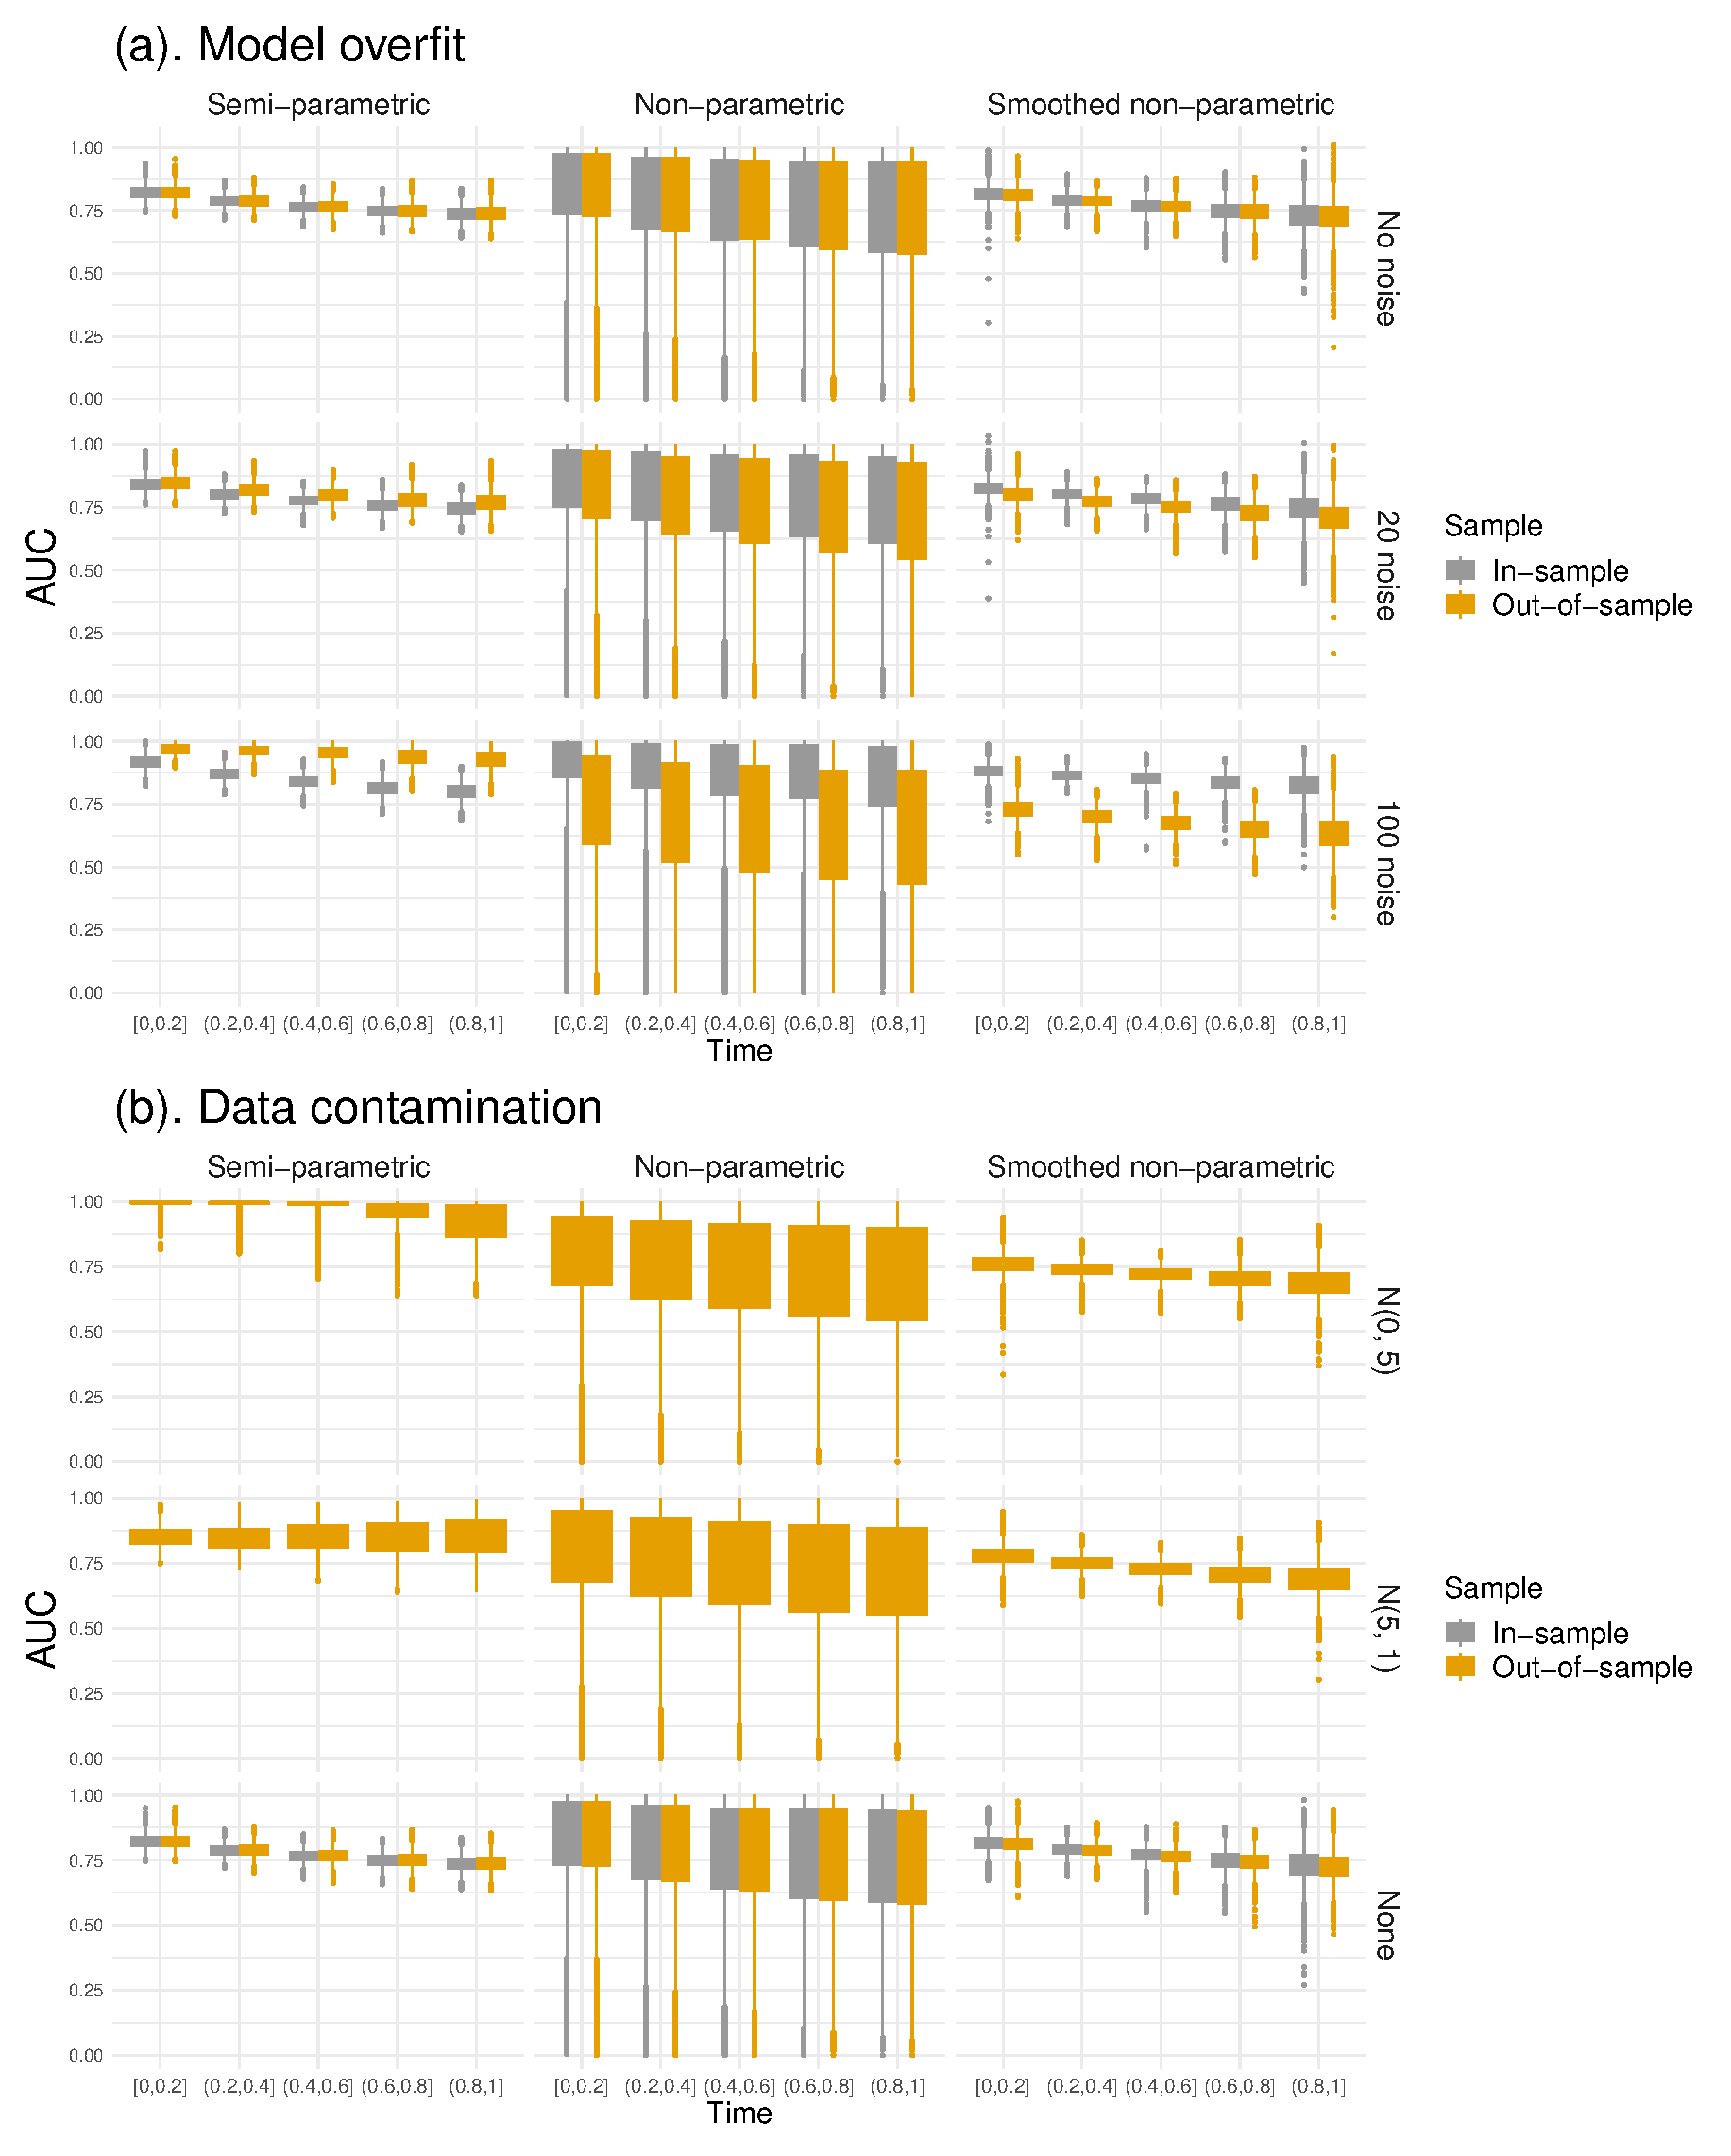
\includegraphics[width=\textwidth]{auc_box.eps}}
    \caption{Comparing variability of in-sample and out-of-sample Incident/Dynamic AUC estimates. The entire follow-up period is divided into five equal-length intervals, and each box represents AUC estimates in the corresponding time interval. Grey boxes represent in-sample estimates, and yellow boxes represent out-of -sample estimates.}
    \label{fig:auc_box}
\end{figure}



\subsection{Mechanism for Inflated Estimation of Out-of-Sample Discrimination}

As described in Section~\ref{subsec:methods_mechanism}, the cause of the observed out-of-sample inflation lies in the semi-parametric estimator of incident sensitivity. Remember the  estimator in Equation~(\ref{eq:sens_sp}) weighs observations at risk at time t by the exponential of their estimated risk scores: 
\[
    \frac{exp(\hat{\eta}_k)}{\sum_{j}I(T_j\geq t)exp(\hat{\eta}_j)}
    %\label{eq:sens_sp_wt}
\]
 

When an observation has a large estimators risk score $\hat{\eta}$, its corresponding weight would also be very large. As a result, the semi-parametric estimator would be dominated by the observations with large estimated risk score, regardless of their actual event status at time $t$ or the accuracy of this risk estimation. In fact, both noise signals and data contamination considered in this simulation study will cause the covariates to be more variable, causing the weight to be very large for a small proportion of subjects. The distribution of this weight on testint samples is visualized in Figure~\ref{fig:np_sens_wt} as a visual representation.

\begin{figure}
    \centerline{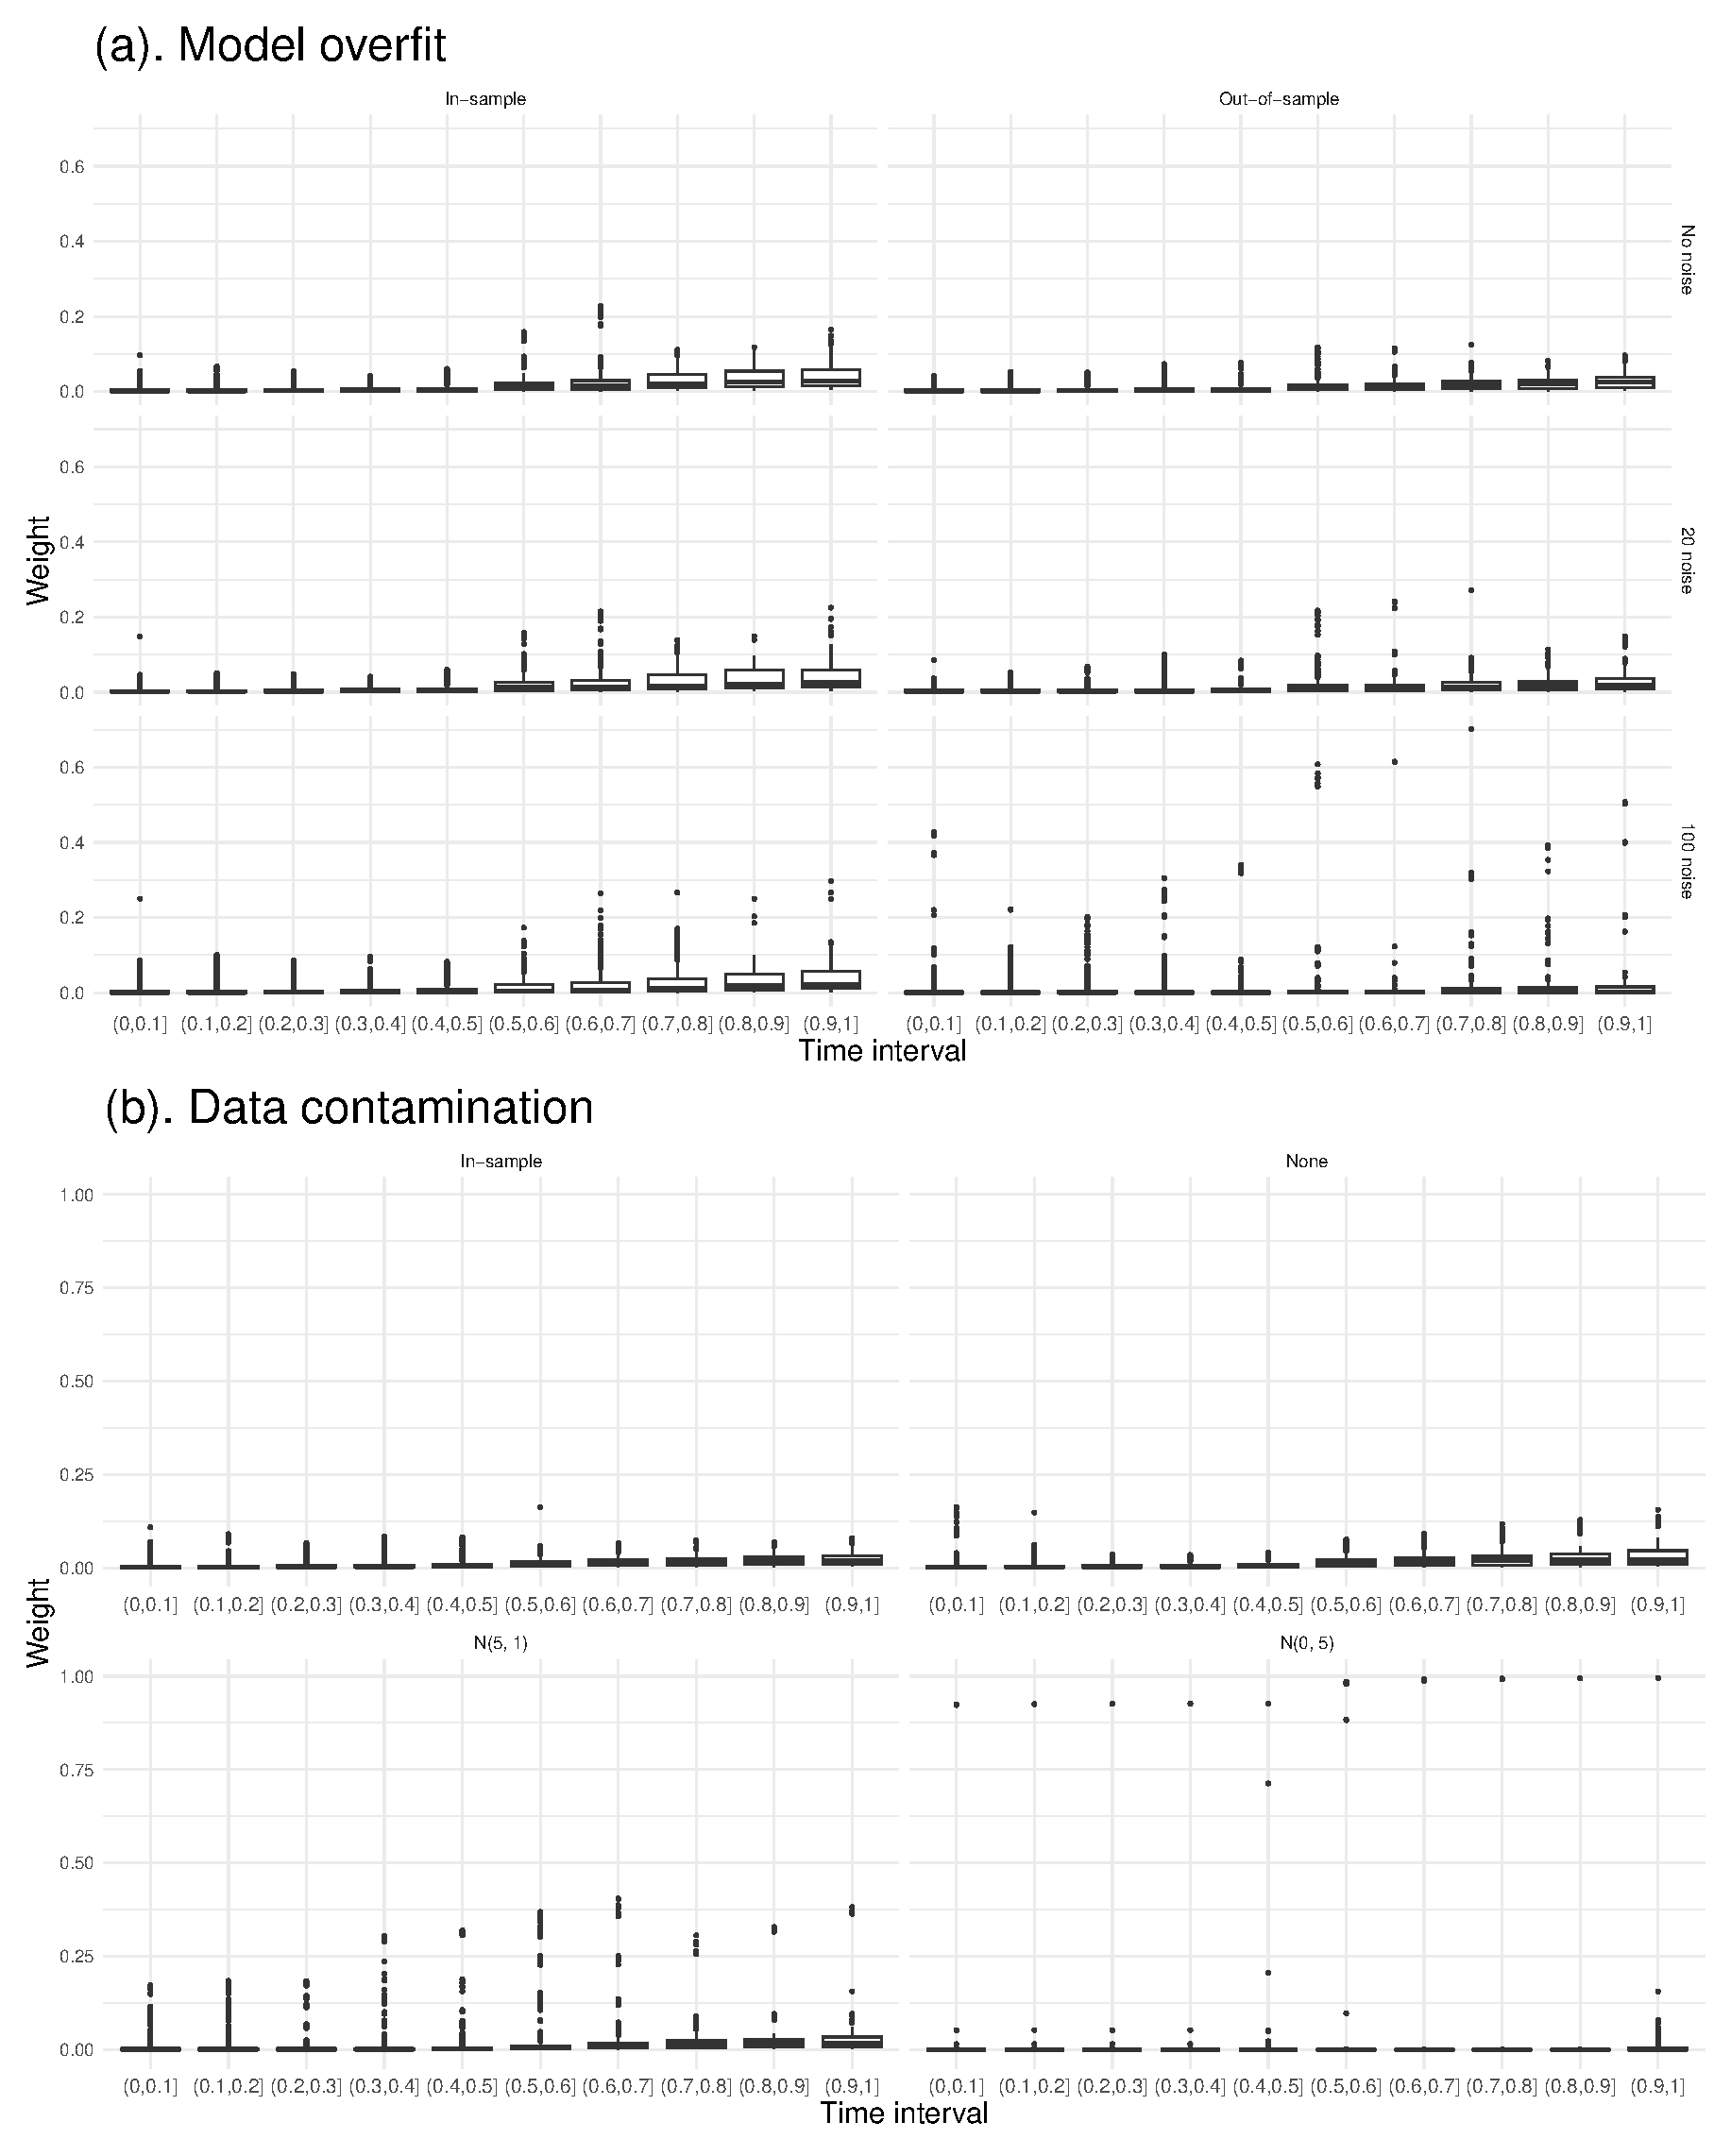
\includegraphics[width=
    \textwidth]{sens_wt.eps}}
    \caption{Distribution of weights in the estimator of incident sensitivity from the simulation study. Subjects are collapsed into equal-length bins across the follow-up period for better visualization.}
    \label{fig:np_sens_wt}
\end{figure}

From Figure~\ref{fig:np_sens_wt}(a) it is easy to see how the additional noise signals has caused the weights to spread a lot higher for some observations in the test samples. When the model is moderately overfit with 20 noise signals (middle-right panel), the highest weight is close to 0.3. However with the severely overfitted model with 100 noise signals (lower-right penal), the weights can end up as high as 0.7. This also explains why the out-of-sample inflation from semi-parametric estimators of $AUC^{I/D}$ and concordance would increase with number of noise signals in the model. Similarly, Figure~\ref{fig:np_sens_wt}(b) shows the values of weight when 10\% of the testing samples is contaminated. A mean shift of covariate distribution (lower-left panel) induced larger weights for these outlying observations. However, the increase of weights is much more significant when the outlying covariates have a larger variance (lower-right penal). For some observations here, the weights go up to close to 1, meaning the sensitivity estimation depends almost entirely on these observations at some time points. 

\section{Data Application}
\label{sec:nhanes_data}
In this section, we present a real-data example of out-of-sample overestimation of discriminative performance from semi-parametric estimators. Specifically, we used data from the National Health and Nutrition Examination Survey (NHANES) from the year 2011-2014 to predict all-cause mortality, using physical activity features and demographics. Note that the NHANES study is a multi-stage probabilistic sample from the non-institutionalized US population. Results are thus generalizable when survey sampling methods are accounted for in regression modelling (i.e. survey weights, cluster sampling. etc). As our data application is for illustrative purposes only, we do not account for survey design. We refer interested readers to \citet{Lumley2004}, \citet{KornandGraubard2011}, and \citet{skinner2017} for overviews of survey methodology for regression analyses. 

%\footnote{The data and source code that support the findings of this study are openly available at https://github.com/yingljin/TV-AUC-thesis.git.}

\subsection{NHANES 2011-2014 Data}
 
The analytic sample includes 3556 participants with age 50-80, at least three days of accelerometry data with 95\% estimated wear time, and complete data in covariates of interest. The total number of observed all-cause mortality events was 424, with a total of 23587.17 person-years of follow-up. Accelerometry data was processed in this spirit of the pipeline used by \citet{glaa250} for the NHANES 2003-2006 and the UK Biobank data, respectively. The predictor vector $\boldsymbol{X_i}$ included five variables: age, BMI, active-to-sedentary transition probability (ASTP), relative amplitude (RA),  and total MIMS units (TMIMS). The latter three variables (ASTP, RA, and TMIMS) are variables derived from participants' wearable accelerometry data. These five variables exhibit moderate pairwise correlation. 

\subsection{Models}
\label{subsec:appl_model}

As the simulation study, we would like to compare the in-sample and out-of-sample behavior of semi- and non-parametric estimators on this real dataset. Specifically, we would like to examine if these estimators could help identify a proper model from a overfitted model. Accordingly, we set up two different Cox models to predict time to mortality. The first model is an additive Cox model as follows: 
\begin{equation}
\log\lambda(t|\bmath{X}_i) = \log \lambda_0(t) + f(\bmath{X}_i) 
    \label{eq:acm}   
\end{equation}

The risk score in this model, $f(\cdot)$, is a smooth function of predictors modelled as a linear combination of $200$ unpenalized thin plate regression splines \citep{wood2003} via the {\it mgcv} package \citep{wood2017} in {\it R} \citep{Rsoftware}. This model which contains a five-dimensional smooth function estimated using $200$ unpenalized spline basis functions (200 coefficients without regularization) will thus tend to substantially overfit to the data. We will refer to Model~(\ref{eq:acm}) as the "additive Cox model" (ACM).

The second model has a simpler linear form for the risk score. Specifically, the second estimated Cox model is:  
\begin{align}
    \log\lambda(t|\boldsymbol{X_i}) &= \log \lambda_0(t) + \boldsymbol{X}_i\boldsymbol{\beta} 
    \label{eq:lcm}
\end{align}
Given the size of the data and the number of observed events, a linear model of this form will tend not to result in overfitting, particularly in comparison to the ACM (Model~\eqref{eq:acm}) presented above. We will refer to Model~\eqref{eq:lcm} as the ``linear Cox model" (LCM).

The discriminative performance of the ACM and LCM models are evaluated using 10-fold cross validation, using both semi- and non-parametric estimators. The former includes Heagerty \& Zheng estimators of Incident/Dynamic AUC and concordance, as well as Gonen \& Heller concordance estimator. The latter refers to non-parametric and smoothed non-parametric estimators of Incident/Dynamic AUC, their corresponding concordance (weighted by smoothed survival function) and Harrell's C index.   



\subsection{Results}
\label{subsec:application_results}

Figure \ref{fig:appl} presents the in- and out-of-sample estimates of $AUC^{I/D}(t)$ and concordance for the simpler LCM and the more complex ACM by various estimators. In (a), the estimates of $AUC^{I/D}$ are smoothed across the folds used for cross validation. We note a few key findings. First, the in-sample and out-of-sample $\hat{AUC}^{I/D}(t)$ are very similar for the linear cox model (yellow lines) for both semi-parametric (left panel) and smoothed non-parametric (right panel) estimator throughout the follow-up period, indicating no overfit in the simpler model. In contrast, there is a marked discrepancy between in- and out-of-sample estimates for the semi-parametric estimator and both non-parametric estimators. Crucially, when comparing out-of-sample estimates, the semi-parametric estimates are much higher that its corresponding in-sample values, while the non-parametric estimators had lower out-of-sample values. 

\begin{figure}
    \centerline{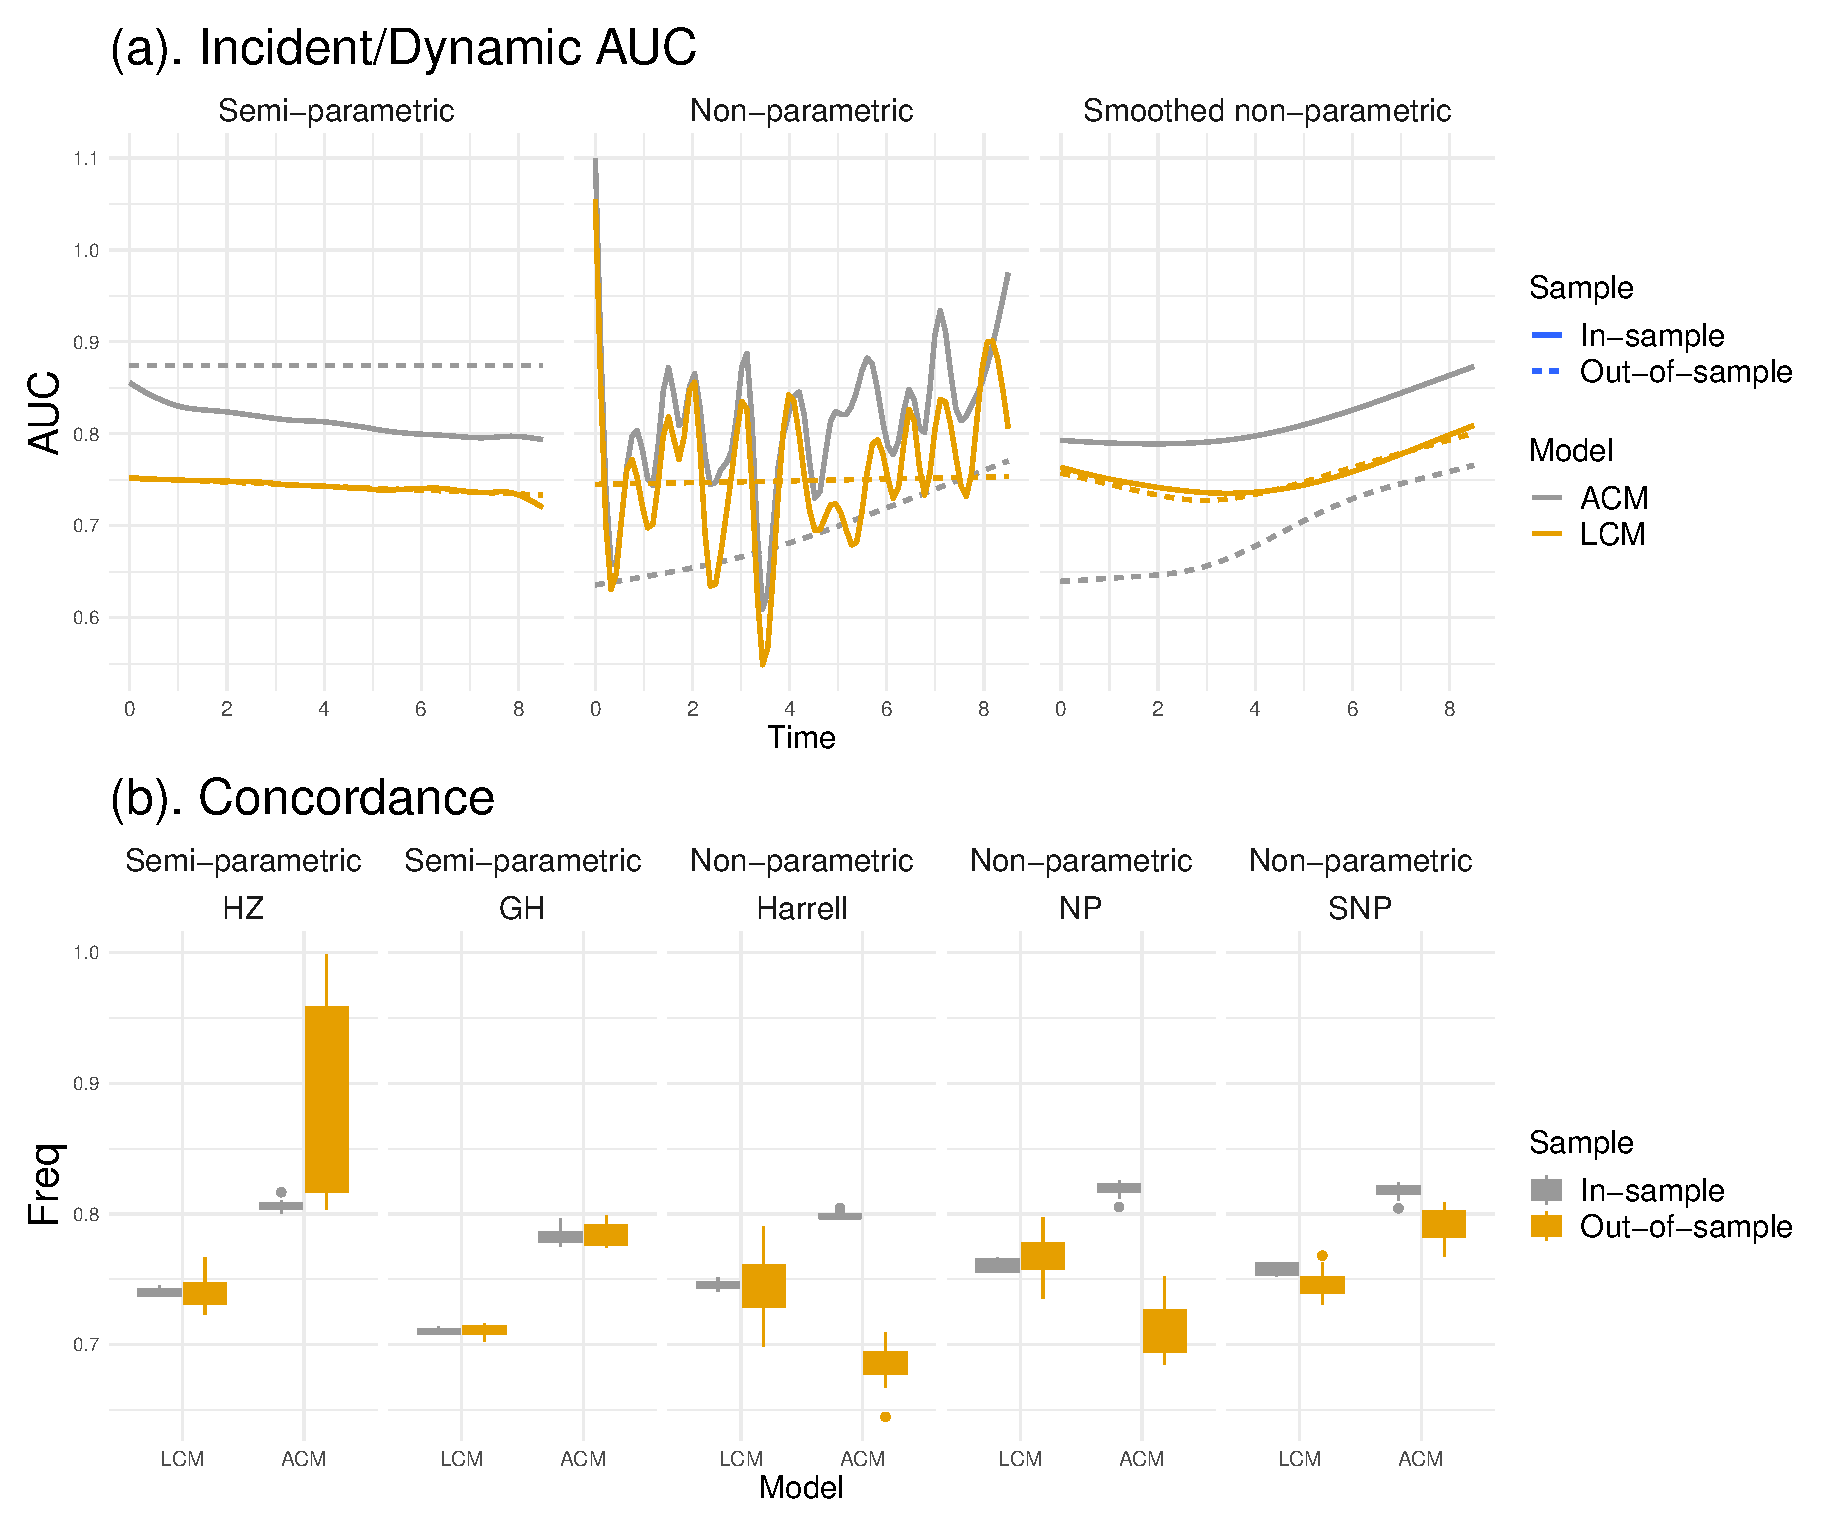
\includegraphics[width=\textwidth]{appl.eps}}
    \caption{Incident/Dynamic AUC and concordance estimates on NHANES data. For Incident/Dynamic AUC estimates in (a), grey indicate the complicated additive Cox model and yellow the simple linear Cox model; solid lines indicate in-sample and dashed lines indicate out-of-sample estimates. For concordance estimates in (b), grey indicates in-sample while yellow out-of-sample estimates.}
    \label{fig:appl}
\end{figure}

The non-parametric estimators behave consistently with the expectation of overfitted models, but the semi-parametric estimator clearly does not reflect the model discrimination ability properly. The difference in out-of-sample semi-parametric $\hat{AUC}^{I/D}(t)$ between two models is striking, with a difference of nearly $0.15$ across the follow-up period ($\approx 0.75$ vs $\approx 0.9$). Indeed, this difference would lead an analyst to choose the more complicated, markedly overfit ACM over the simpler LCM if they were to use the semi-parametric estimator with cross-validation for model selection. 

As an aside, the highly non-linear shape of the in-sample non-parametric estimator of $\hat{AUC}^{I/D}(t)$ (middle panel) for the LCM and ACM appears to be driven by a high degree of inconsistency in the estimator at each time point. This finding should not be over-interpreted, and may simply be an artifact of the data and the highly variable nature of the non-parametric estimator. 

The same out-of-sample inflation is also observed in Concordance estimators, as in Figure~\ref{fig:appl} (b). Specifically, semi-parametric and non-parametric estimators show similar in-sample behavior, with in-sample estimates to be higher for the ACM compared to the LCM. In contrast, out-of-sample concordance is inflated (mean Heagerty \& Zheng $C=0.877$) or unchanged (mean Gonan \& Heller $C = 0.785$) from the in-sample estimates for semi-parametric estimators, while non-parametric estimators show the expected drop (mean non-parametric $C=0.712$, smoothed non-parametric $C=0.791$, Harrell's $C=0.683$). Again, these results would lead an analyst to choose the more complex ACM, despite overfitting to the data, over the LCM when using cross-validated semi-parametric concordance as a model selection criteria. 

\section{Discussion}
\label{sec:discussion}

Our investigation of the properties of semi- and non-parametric estimators of Incident/Dynamic AUC and the corresponding estimators of Concordance indicate that out-of-sample estimators suffer from an intrinsic tendency to overestimate model discrimination when applied to samples not used to fit the data. Here, we have identified, characterized, and quantified the nature of this phenomena through both a simulation study and case study on real-world data. This property calls into serious question the appropriateness of this class of semi-parametric estimators for model comparison/selection purposes, particularly when comparing complicated models to simple models. Moreover, this phenomena is likely to occur when applied to a new sample whose covariate space does not overlap well with training data, even when the model is correctly specified. 

The behavior we identified suggests that non-parametric estimators should generally be preferred over semi-parametric estimators of Incident/Dynamic discrimination. However, non-parametric estimators are highly variable due to the relatively small number of events at any given time point, motivating the need for a smoothed estimator. As such, we proposed a method for smoothing these non-parametric estimators using penalized regression splines, though other smoothers (e.g. kernel smoothing) may be used. In our simulation study, the penalized regression spline approach worked well for reducing variability, but resulted in slight bias. This is likely due to heteroskedasticity of the residual process and correlation of estimates for $AUC(t)$ along $t$ which are not accounted for in classical additive models. Further methodologic work for identifying optimal smooth estimators and establishing accurate inferential procedures is needed. 

In summary, this work represents an important step forward in identifying the conditions under which various estimators of discrimination in time-to-event models are appropriate. Critically, we identify a property intrinsic to many semi-parametric estimators for Incident/Dynamic AUC and their resulting estimates of Concordance which indicates their unfitness for assessing out-of-sample discrimination. Lastly, we provide evidence to support the use of smoothed versions of non-parametric estimates of time-dependent AUC for model comparison purposes.  

% \section{Inference}
% \label{s:inf}

% Please see the file \texttt{biomsample.tex} for fancy examples of making
% tables.  Here is a very simple one.  Use \texttt{table} for tables
% that are narrow enough to fit in one column of the typeset journl; use
% \texttt{table*} for tables that need to span two columns.  For
% figures, use of \texttt{figure} and \texttt{figure*} is analogous. 

% \begin{table}
% \caption{This is a simple table.}
% \label{t:one}
% \begin{center}
% \begin{tabular}{lrrr}
% \Hline
% Estimator & \multicolumn{1}{c}{$\beta_1$} &  \multicolumn{1}{c}{$\beta_2$} & 
% \multicolumn{1}{c}{$\beta_3$} \\ \hline
% MLE & 10.18 & $-$3.26 & 0.13 \\
% OLS & 9.92 & $-$3.19 & 0.11 \\
% WLS & 9.88 & $-$3.33 & 0.12 \\
% \hline
% \end{tabular}
% \end{center}
% \end{table}

% You can experiment with fancier tables than Table~\ref{t:one}.

% We can get bold symbols using \verb+\bmath+, for example, $\bmath{\alpha}_i$.

% \section{Discussion}
% \label{s:discuss}

% Put your final comments here. 

% %  The \backmatter command formats the subsequent headings so that they
% %  are in the journal style.  Please keep this command in your document
% %  in this position, right after the final section of the main part of 
% %  the paper and right before the Acknowledgements, Supporting Information (Supplementary %  Materials),   and References sections. 

% \backmatter

% %  This section is optional.  Here is where you will want to cite
% %  grants, people who helped with the paper, etc.  But keep it short!

% \section*{Acknowledgements}

% The authors thank Professor A. Sen for some helpful suggestions,
% Dr C. R. Rangarajan for a critical reading of the original version of the
% paper, and an anonymous referee for very useful comments that improved
% the presentation of the paper.\vspace*{-8pt}



%  Here, we create the bibliographic entries manually, following the
%  journal style.  If you use this method or use natbib, PLEASE PAY
%  CAREFUL ATTENTION TO THE BIBLIOGRAPHIC STYLE IN A RECENT ISSUE OF
%  THE JOURNAL AND FOLLOW IT!  Failure to follow stylistic conventions
%  just lengthens the time spend copyediting your paper and hence its
%  position in the publication queue should it be accepted.

%  We greatly prefer that you incorporate the references for your
%  article into the body of the article as we have done here 
%  (you can use natbib or not as you choose) than use BiBTeX,
%  so that your article is self-contained in one file.
%  If you do use BiBTeX, please use the .bst file that comes with 
%  the distribution.  In this case, replace the thebibliography
%  environment below by 
%
\bibliographystyle{biom} 
\bibliography{refs}
\nocite{*}

% \begin{thebibliography}{}

% \bibitem{ } Cox, D. R. (1972). Regression models and life tables (with
% discussion).  \textit{Journal of the Royal Statistical Society, Series B}
% \textbf{34,} 187--200.

% \bibitem{ }  Hastie, T., Tibshirani, R., and Friedman, J. (2001). \textit{The 
% Elements of Statistical Learning: Data Mining, Inference, and Prediction}.
% New York: Springer.

% \end{thebibliography}

%  If your paper refers to supporting web material, then you MUST
%  include this section!!  See Instructions for Authors at the journal
%  website http://www.biometrics.tibs.org



\appendix

%  To get the journal style of heading for an appendix, mimic the following.

\section{Evaluating True I/D AUC}
We can obtain true incident sensitivity and dynamic specificity under our data generating mechanism by monte-carlo integration. Specifically, consider incident sensitivity
\begin{align*}
    \text{Pr}(\eta > c|T = t) 
    &= E[1(\eta > c) | T = t] \\
    &= \int 1(\eta > c) f(\eta | t) d\eta \\
    &= \int 1(\eta > c) \frac{f(t|\eta)f(\eta)}{\int f(t|\eta) f(\eta)d\eta}d\eta
\end{align*}
Since $\eta = \bm{x}^t \bm{\beta}$ is a linear combination of normal random variables, 
$\eta$ is normally distributed. In addition, under the assumption of a Weibull baseline hazard, we can obtain 
\begin{align*}
    f( t| \eta) 
    &= \lambda(t|\eta)S(t|\eta) \\
    &= (\theta e^{\eta})p t^{p-1} e^{-(\theta e^{\eta}) t^p }
\end{align*}
We can then estimate incident sensitivity using numeric integration via, e.g., the {\it integrate()} function in {\it R}.

Next, consider dynamic specificity
\begin{align*}
    \text{Pr}(\eta \leq c|T > t) 
    &= \frac{\text{Pr}(\eta \leq c \cap T > t)}{\text{Pr}(T > t) } \\
    % &= \frac{\text{Pr}(T_i > t|\eta_i \leq c )\text{Pr}(\eta_i \leq c)}{\text{Pr}(T_i > t) } \\
    % &= \frac{\text{Pr}(T_i > t|\eta_i \leq c )\int_{-\infty}^c f(\eta)d\eta}{\int_t^\infty f(t)dt } \\
    &= \frac{\int_t^\infty \int_{-\infty}^c f(t,\eta)d\eta dt }{\int_t^\infty [\int f(t|\eta)f(\eta)d\eta]dt } \\
        &= \frac{\int_t^\infty \int_{-\infty}^c f(t|\eta)f(\eta) d\eta dt }{\int_t^\infty [\int f(t|\eta)f(\eta)d\eta] dt} \\
\end{align*}
The double integrals involved can again be evaluated using numeric integration via, e.g., the {\it cubature::adaptIntegrate()} function in {\it R}.


%\section{Variability of Estimators of Incidenct/Dynamic AUC}





% \section*{Supporting Information}

% Web Appendix A, referenced in Section~\ref{s:model}, is available with
% this paper at the Biometrics website on Wiley Online
% Library.\vspace*{-8pt}



% review and follow the journal policy for this material, available
% under Instructions for Authors at \texttt{http://www.biometrics.tibs.org}.

\label{lastpage}

\end{document}
